
\section{Experiment Setup}
\begin{figure*}
	\centering
	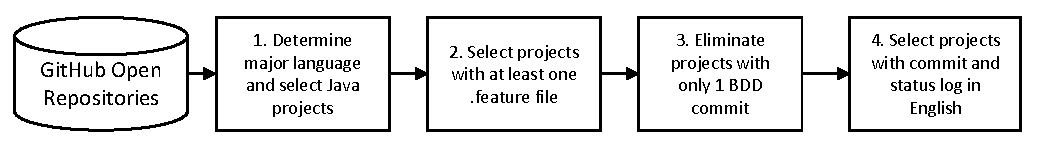
\includegraphics[height=0.9in, width=6.6in]{exp_setup.pdf}
	\caption{An overview of the experiment design}
\end{figure*}
In this section, we explain how we collect the data used for answering our research questions.

Figure 3 shows an overview of our entire experiment setup process. In \textbf{Step 1}, we use the GitHub search API to find project that mainly uses Java. We choose Java because the BDD framework \textit{Cucumber} for Java is currently the most popular BDD tool \cite{BDDFrame}. Filtering Java projects is done by the search API of GitHub. Using the API, we can identify the major language of a project. GitHub uses the \textit{Linguist} library to identify the major language in each project. Our search retrieves 1,005,247 projects in total and we extract 59,933 Java projects amongst all the retrieved projects. In \textbf{Step 2}, we use the tree API in GitHub to find projects that include at least one \textit{.feature} file, which we deem as a BDD project. We find that 927 out of 59,933 projects actually contain \textit{.feature} files. In \textbf{Step 3}, we filter out the projects that contain only one commit manipulating a \textit{.feature} file to avoid projects that do not actually use BDD. After this filtering, 890 projects survive. In \textbf{Step 4}, we eliminate BDD projects that do not have both \textit {commit log} and \textit {status} data in English. Commit logs provide information regarding every modification to the project (e.g., why certain files are modified). The status data stores the status of every commit, i.e., author, date and modified files. For our research, it is important for the information to be in English to understand the purpose of each commit and to make our research more reproducible. Also, we perform text processing with regards to English words in RQ1, so projects with information in a foreign language (e.g., Arabic) would hinder our analyses. In the end, 133 BDD projects remain. We highlight some key characteristics of our studied projects by selecting 50 of our 133 BDD projects with the highest total LOC. Table 1 shows the year created, total commits, total pull requests, total forks and total stars for each of our studied projects.

\begin{table*}
	\normalsize
	\caption{Characteristics of 50 studied BDD projects}
	\center
	
	\begin{tabular}{p{6cm} c c c c c}
		\textbf{Project} (Username/Project-Name) & \textbf{Year Created} & \textbf{Total commits} & \textbf{Pull requests} & \textbf{Forks} & \textbf{Stars}\\
		\hline
tyen/cs320tests & 2009 & 207 & 0 & 0 & 9 \\
caspian311/Scripturelookup & 2009 & 109 & 0 & 0 & 2 \\
epabst/expressive & 2009 & 72 & 0 & 1 & 3 \\
epabst/expressiveBDD & 2009 & 46 & 0 & 2 & 2 \\
mkristian/slf4r & 2009 & 41 & 0 & 0 & 6 \\
Vaysman/jvote & 2009 & 29 & 0 & 0 & 0 \\
Serabe/javascreepy & 2009 & 22 & 0 & 0 & 1 \\
rapidftr/RapidFTR-Android & 2010 & 1214 & 31 & 83 & 38 \\
davidbkemp/nate & 2010 & 259 & 0 & 0 & 0 \\
jtigger/kanban-simulator & 2010 & 196 & 0 & 0 & 4 \\
yujunliang/lambda & 2010 & 83 & 0 & 0 & 8 \\
jacek99/maven-python-mojos & 2010 & 73 & 1 & 12 & 18 \\
rapaul/cuke4ninja & 2010 & 70 & 0 & 0 & 1 \\
trevershick/jook & 2010 & 69 & 2 & 2 & 1 \\
sveinung/pritest-server & 2010 & 57 & 1 & 0 & 6 \\
openengsb-labs/labs-yaste & 2010 & 32 & 0 & 1 & 3 \\
runeflobakk/poker & 2010 & 27 & 0 & 1 & 1 \\
bugsnag/bugsnag-android & 2011 & 645 & 29 & 154 & 872 \\
AndreasWilhelm/neo4j-spatial & 2011 & 360 & 0 & 0 & 2 \\
resthub/springmvc-router & 2011 & 214 & 29 & 59 & 170 \\
rlogiacco/SmartUnit & 2011 & 178 & 5 & 5 & 15 \\
vitormcruz/payroll\_cs & 2011 & 173 & 0 & 0 & 2 \\
mkristian/rails-resty-gwt & 2011 & 164 & 0 & 2 & 12 \\
akollegger/trivial-graph & 2011 & 85 & 0 & 0 & 1 \\
jfinkhaeuser/androdyne & 2011 & 64 & 0 & 0 & 5 \\
Drin/spam & 2011 & 50 & 0 & 1 & 1 \\
dokipen/embedly-java & 2011 & 39 & 1 & 9 & 1 \\
jescov/jescov & 2011 & 39 & 0 & 4 & 10 \\
jkransen/treemarks & 2011 & 38 & 0 & 0 & 0 \\
Jennifer-fu/practices & 2011 & 36 & 0 & 0 & 1 \\
lukasz-kaniowski/cucumber-selenium-rc & 2011 & 33 & 0 & 1 & 2 \\
ZsoltFabok/cucumber-jvm-post & 2011 & 22 & 0 & 10 & 17 \\
Chorus-bdd/Chorus & 2012 & 1124 & 17 & 9 & 35 \\
bartbaas/spatial & 2012 & 565 & 0 & 0 & 2 \\
daniel-andersen/Q-Cumberless-Testing & 2012 & 348 & 0 & 0 & 4 \\
leviwilson/oasis-android & 2012 & 244 & 0 & 0 & 1 \\
tlauchenauer/gaia-pdb & 2012 & 237 & 0 & 0 & 1 \\
bclozel/springmvc-router & 2012 & 214 & 2 & 7 & 42 \\
rabid-fish/JavaTechExamples & 2012 & 178 & 0 & 0 & 1 \\
iantmoore/old-substeps-webdriver & 2012 & 163 & 0 & 1 & 1 \\
ericlemerdy/one-kata-per-day & 2012 & 118 & 0 & 3 & 7 \\
mikael-wilhelm/LoadPlannerAmaz & 2012 & 109 & 0 & 0 & 1 \\
marky-mark/MTT & 2012 & 77 & 0 & 0 & 1 \\
leefaus/soa-petstore & 2012 & 56 & 0 & 4 & 4 \\
suggitpe/java-web & 2012 & 40 & 0 & 1 & 0 \\
japonophile/jescov & 2012 & 39 & 0 & 0 & 1 \\
sandromancuso/tww-java & 2012 & 33 & 0 & 0 & 2 \\
ilanpillemer/gherkin-eclipse-plugin & 2012 & 26 & 0 & 2 & 18 \\
talios/cucumber-testng-factory & 2012 & 26 & 3 & 9 & 13 \\
hayatoshimizuBSKYB/apollo & 2012 & 23 & 3 & 1 & 5

	\end{tabular}
\end{table*}
